% document formatting
\documentclass[10pt]{article}
\usepackage[utf8]{inputenc}
\usepackage[left=1in,right=1in,top=1in,bottom=1in]{geometry}
\usepackage[T1]{fontenc}
\usepackage{xcolor}

% math symbols, etc.
\usepackage{amsmath, amsfonts, amssymb, amsthm}

% lists
\usepackage{enumerate}
\usepackage{tabularx}

% images
\usepackage{graphicx} % for images
\usepackage{tikz}

% code blocks
% \usepackage{minted, listings} 

% verbatim greek
\usepackage{alphabeta}

\graphicspath{{./assets/images/Module 4}}

\title{02-680 Module 4 \\ \large{Essentials of Mathematics and Statistics}}
 
\author{Aidan Jan}

\date{\today}

\begin{document}
\maketitle

\section*{Graphs}
\textbf{Graphs} are powerful tools for modeling structured \textbf{relationships} between entities.  A graph consists of:
\begin{itemize}
	\item \textbf{Nodes} (or Vertices): The entities in the graph
	\item \textbf{Edges} (or Links): The relationships between pairs of nodes.
\end{itemize}
A graph is also called a \textbf{network}.

\subsection*{Undirected Graphs}
\begin{itemize}
	\item In \textbf{undirected graphs}, edges represent mutual relationships.  If node $A$ is connected to node $B$, then node $B$ is also connected to node $A$.
\end{itemize}
Many real-world relationships are mutual.  This representation is suitable for systems where all connections are peer-to-peer.

\subsection*{Directed Graphical Models}
In a social network, each \textbf{node} represents a person, and each \textbf{directed edge} represents a relationship such as following, influencing, or messaging.  These directed connections capture how information, behavior, or influence propagates across the network.

\subsection*{Directed Graph vs. Undirected Graph}
In a directed graph, an edge is an \textbf{ordered pair} of vertices ("an edge from $u$ to $v$") and in an undirected graph, an edge is an unordered pair of vertices ("an edge between $u$ and $v$").
\begin{center} 
	\includegraphics*[width=0.7\textwidth]{M4_1.png} 
\end{center}
\rule{\textwidth}{0.4pt}
\par
\pagebreak
A \textbf{graph} is a mathematical structure used to model pairwise relationships.  We typically write a graph as a tuple $G = \langle V, E \rangle$.
\begin{itemize}
	\item $V$ is a set of nodes or vertices
	\item $E$ is a set of edges, each connecting a pair of nodes.
	\begin{itemize}
	    \item $E \subseteq V \times V$ if $G$ is \textbf{directed}
	    \item $E \subseteq \{\{u, v\} \::\: u, v \in V\}$ if $G$ is \textbf{undirected}
	    \item Note that one edge can loop around the same node.  (e.g., $u = v$)
    \end{itemize}
\end{itemize}
Nodes in a graph are typically drawn as circles ad edges are represented as lines.  In directed graphs, each edge is drawn with an arrow indicating its orientation ("which way it goes").

\subsection*{Parents and Children}
In a directed graph, there exists the notion of parent nodes and child nodes.  If an arrow connects two variables $X$ and $Y$ (in either direction) we say that $X$ and $Y$ are adjacent.  If there is an arrow from $X$ to $Y$, then $X$ is a parent of $Y$, and $Y$ is a child of $X$.  A \textbf{directed path} between two variables is a set of arrows all pointing in the same direction linking one variable to the other such as:
\begin{center} 
	\includegraphics[width=0.6\textwidth]{M4_2.png}
\end{center}

\subsection*{Some Examples of Graphs}
To understand a \textbf{directed graph}, think about the difference between:
\begin{itemize}
	\item Twitter follows: $A \rightarrow B$ (directed)
	\item Facebook friendships: $A - B$ (undirected)
\end{itemize}
\begin{center} 
	\includegraphics*[width=0.9\textwidth]{M4_3.png} 
\end{center}

\subsection*{Path in a Directed Graph}
Some examples of things that can be represented as \textbf{graphs}: train/flight maps, cell interactions, social networks, etc.  A \textbf{path} is a sequence of nodes:
\[\langle v_1, v_2, v_3, \dots, v_k \rangle\]
\begin{center}
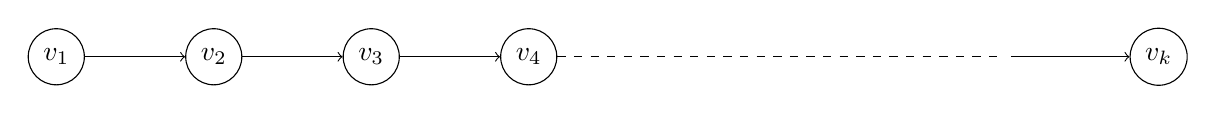
\begin{tikzpicture}
    \node[draw, circle] at (0, 0) (1) {$v_1$};
    \node[draw, circle] at (2, 0) (2) {$v_2$};
    \node[draw, circle] at (4, 0) (3) {$v_3$};
    \node[draw, circle] at (6, 0) (4) {$v_4$};
    \node at (12, 0) (dots) {};
    \node[draw, circle] at (14, 0) (k) {$v_k$};
    \draw[->] (1) edge (2);
    \draw[->] (2) edge (3);
    \draw[->] (3) edge (4);
    \draw[dashed] (4) edge (12, 0);
    \draw[->] (dots) edge (k);
\end{tikzpicture}
\end{center}
\begin{itemize}
	\item $\langle v_i, v_{i + 1} \rangle \in E$ if $G$ is \textbf{directed}
	\item $\{v_1, v_{i + 1}\} \in E$ if $G$ is \textbf{undirected}
\end{itemize}
We say that the \textbf{path} has length $k$, and that a path is from $v_1$ to $v_k$.

\subsection*{Route Graph}
In the case of a route graph (e.g., for navigation or delivery), each edge might be labeled with a street name (a string), but in other types of graphs the labels could be numerical values (such as distance, time, or cost) - which we usually call \textbf{weights}.\\
\begin{itemize}
	\item A \textbf{path label} could be the concatenation of street names (e.g. "Main St." \textrightarrow "Broadway" \textrightarrow "5th Ave.")
	\item A \textbf{path weight} could be the \textbf{sum} of distnaces or travel time along the path.  Edge labels can carry qualitative (string) or quantitative (numeric) information, and we interpret paths differently depending on the type of label.
\end{itemize}

\subsection*{Graph Function}
We can also \textbf{label} or \textbf{weight edges} in some scenarios.  What does this mean?
\begin{itemize}
	\item In many types of graphs (especially weighted or labeled graphs) we want to assign a value or label to each edge.
	\item These labels can be:
	\begin{itemize}
	    \item Strings (e.g., street names, course codes, etc.)
	    \item Numbers (e.g., cost, distance, weight, time)
    \end{itemize}
\end{itemize}
Formally, edges with string labels are typically represented by a function:
\[\ell \::\: E \rightarrow \Sigma\]
(or maybe edges with weight labels function $w \::\: E \rightarrow \mathbb{R}$)\\\\
Instead of assigning labels manually, we define a \textbf{function} that maps each edge to a value.
\begin{center}
    \begin{tabularx}{\textwidth}{XXX}
    \textbf{Function} & \textbf{Purpose} & \textbf{Output Type} \\
    $\ell$ & Edge label & A string (from $\Sigma^*$) \\
    $w$ & Edge weight & A real number ($\mathbb{R}$)
    \end{tabularx}
\end{center}

\subsection*{Neighborhood of a Node: Undirected Graph}
Let $G = \langle V, E \rangle$ be an \textbf{undirected graph}, and let $u \in V$ be a \textbf{node}.  The neighborhood of $u$ is the set $v \in V \::\: \{u, v\} \in E$.
\begin{itemize}
	\item That is, the set of all neighbors of $u$
\end{itemize}
$N_G(v)$ is the set of all nodes $u$
\begin{itemize}
	\item If $\{u, v\} \in E$, it means there is an edge connecting $u$ and $v$, so node $u$ is considered a neighbor of node $v$.
\end{itemize}

\subsection*{Degree: Undirected Graph}
The \textbf{degree} of a node $u$ is an undirected graph $G$ is the size of the neighborhood of $u$ in $G$, that is, the number of nodes adjacent to $u$.

\subsubsection*{Aside: Indicator Function}
The \textbf{indicator function} is a simple mathematical tool used to express whether a condition is \textbf{true} or \textbf{false}, in a numeraical form.  Given an arbitrary set $X$, the indicator function of a subset $A$ of $X$ is the function:
\[1_A \::\: X \mapsto \{0, 1\}\]
defined by
\[1_A(X) = \begin{cases}1 &\text{ if }x \in A \\ 0 &\text{ if }x \notin A\end{cases}\]






\section*{Complete Graphs: LECTURE ENDED HERE}
\end{document}